\chapter{Conclusions}

\section{Further work}
The Xaviers could be switched out with computers using x86 processor for limiting sources of error. 

\subsection{Improving platooning algorithms}
\paragraph{Time Delay} algorithm is working and can be improved with more information into the "subpub" node. The node can subscribe to odometry of Husky and TB3, and use this information to calculate the offset of where the TB3 is and where it should be. When Husky drives with Nav2 the topic \topic{/path} can be used for improving where the averness of where teh TB3 should be. Potentially LiDAR data can also be used, and the algorithm could be improved forever. Continuing improving on Time Delay feels like building a bad of Nav2. Therefor the author of this thesis believe using Nav2 API is the best way to achieve autonomous platooning with ROS2. 

\paragraph{Nav2 API} has been work on but is not finished as explained in Table \ref{tab:MilestonesNav2API}. The main challenge left is running two robots with Nav2 simultaneously on the same network. It may be that both robots need two be able to run Nav2 with namespace, but probably just one. Launching two robots may be possible with using the standard launch files from Nav2, it is also possible a custom launch file need to be build using Nav2 nodes cindo like this video \cite{MultiRobotNav2}.

\paragraph{AprilTags/ArUco} where researched but not tested. AprilTags and ArUco markers is a system where a camera can get a tf from viewing the tag seen in Figure \ref{fig:apriltags} and demonstrated in Figure \ref{fig:apriltag_principal}. When a tf between TB3 and Husky is acquired this can be used to make a platooning system or improve on an existing one. 

\begin{figure}[H]
  \centering
  \begin{minipage}[b]{0.4\textwidth}
    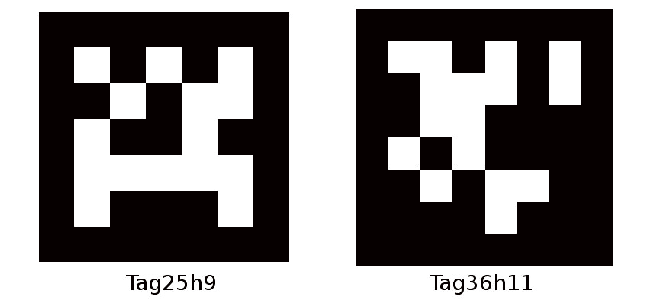
\includegraphics[width=\textwidth]{Figures/images/apriltags.png}
    \caption{Example of two AprilTags}
    \label{fig:apriltags}
  \end{minipage}
  \hfill
  \begin{minipage}[b]{0.4\textwidth}
    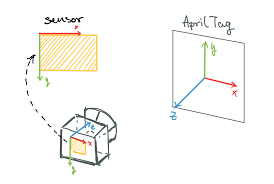
\includegraphics[width=\textwidth]{Figures/images/apriltag_prinsipal.png}
    \caption{Drawing showing the principal of AprilTags}
    \label{fig:apriltag_principal}
  \end{minipage}
\end{figure}
